% TCC: História da Engenharia de Reservatórios (versão ISPTEC - otimizada 15 páginas)
\PassOptionsToPackage{brazilian}{babel}
\documentclass[12pt,a4paper,oneside,brazilian,sumario=tradicional]{abntex2}

% Pacotes básicos e layout ISPTEC
\usepackage[T1]{fontenc}
\usepackage[utf8]{inputenc}
\usepackage{times}
\usepackage{geometry}
\geometry{a4paper,left=3cm,right=2cm,top=3cm,bottom=2cm}
\usepackage{setspace}
\OnehalfSpacing
\usepackage{indentfirst}
\setlength{\parindent}{1.25cm}
\usepackage{emptypage}

% Figuras, tabelas e ilustrações
\usepackage{graphicx}
\usepackage{grffile}
\graphicspath{{figuras/}}
\usepackage{booktabs}
\usepackage{longtable}
\usepackage{array}
\usepackage{multirow}
\usepackage{float}
\usepackage{caption}
\usepackage{wrapfig}
\usepackage{tikz}
\captionsetup{font=small, labelfont=bf, justification=centering, skip=6pt}
\renewcommand{\fonte}[1]{\vspace{2pt}\par\noindent\footnotesize Fonte: #1}

% Matemática
\usepackage{amsmath}
\usepackage{amssymb}
\usepackage{amsfonts}

% Utilitários
\usepackage{hyperref}
\usepackage{xcolor}
\usepackage{enumitem}
\usepackage{lastpage}
\usepackage{microtype}

% Bibliografia ABNT via biblatex
\usepackage[backend=biber,style=abnt]{biblatex}
\addbibresource{referencias.bib}

\hypersetup{
  pdftitle={História da Engenharia de Reservatórios},
  pdfauthor={Grupo 5},
  colorlinks=true,
  linkcolor=black,
  citecolor=black,
  urlcolor=black
}

\DeclareOldFontCommand{\tt}{\normalfont\ttfamily}{\texttt}
\usepackage{url}
\providecommand{\htmladdnormallink}[2]{\href{#2}{#1}}

% Dados do trabalho
\titulo{A história de engenharia de reservatórios de petróleo}
\autor{Grupo 5}
\orientador{Prof.\ Geraldo André Raposo Ramos}
\instituicao{Instituto Superior Politécnico de Tecnologias e Ciências -- ISPTEC\\Departamento de Geociências\\Curso de Engenharia de Petróleo}
\local{Luanda -- Angola}
\data{2026}
\tipotrabalho{Trabalho de Avaliação Contínua}
\preambulo{Trabalho investigativo apresentado ao Curso de Engenharia de Petróleo do Departamento de Geociências do Instituto Superior Politécnico de Tecnologias e Ciências (ISPTEC) como avaliação contínua na disciplina de Engenharia de Reservatórios.}

\begin{document}
\frenchspacing
\pretextual

% ===========================
% CAPA CUSTOMIZADA CONFORME NORMAS ISPTEC
% ===========================
\thispagestyle{empty}
\begin{center}
  % Logo ISPTEC no topo
  \vspace*{0.5cm}
  
\includegraphics[width=3.5cm]{logo isptec.png}
  
  \vspace*{0.8cm}
  
  % Cabeçalho com dados da instituição
  {\large\bfseries DEPARTAMENTO DE GEOCIÊNCIAS E TECNOLOGIAS}
  
  \vspace*{0.3cm}
  
  {\large\bfseries CURSO DE ENGENHARIA DE PETRÓLEO}
  
  \vspace*{2.0cm}
  
  % Nome do autor
  {\large\bfseries GRUPO 5}
  
  \vspace*{1.5cm}
  
  % Título do trabalho
  {\bfseries\Large A HISTÓRIA DA ENGENHARIA DE RESERVATÓRIOS DE PETRÓLEO}
  
  \vspace*{3.0cm}
  
  % Espaço para o trabalho
  ~
  
  \vfill
  
  % Rodapé com local e data
  {\large\bfseries Luanda}
  
  {\large\bfseries 2026}
  
  \vspace*{0.5cm}
\end{center}

% Configurar a página para não contar como numerada
\clearpage
\phantomsection

% ===========================
% FOLHA DE ROSTO
% ===========================
\thispagestyle{empty}
\begin{center}
  
  \vspace*{2.0cm}
  
  {\large\bfseries GRUPO 5}
  
  \vspace*{1.5cm}
  
  {\bfseries\Large A HISTÓRIA DA ENGENHARIA DE RESERVATÓRIOS DE PETRÓLEO}
  
  \vspace*{2.0cm}
  
\end{center}

\hspace*{3.5cm}\begin{minipage}[t]{9.5cm}
Trabalho investigativo apresentado ao Curso de Engenharia de Petróleo do Departamento de Geociências do Instituto Superior Politécnico de Tecnologias e Ciências (ISPTEC) como avaliação contínua na disciplina de Engenharia de Reservatórios.

\vspace*{1.0cm}

\noindent Orientador: Prof.\ Geraldo André Raposo Ramos
\end{minipage}

\vspace*{2.0cm}

\begin{center}
  {\large\bfseries Luanda}
  
  {\large\bfseries 2026}
\end{center}

\clearpage

% Folha de aprovação
\begin{folhadeaprovacao}
  \thispagestyle{empty}
  \begin{center}
    {\ABNTEXchapterfont\large\MakeUppercase{\imprimirautor}}
    \vspace*{1cm}
    \begin{center}
      \ABNTEXchapterfont\bfseries\large\MakeUppercase{\imprimirtitulo}
    \end{center}
    \vspace*{1cm}
    \hspace{.38\textwidth}
    \begin{minipage}{.56\textwidth}
      \imprimirpreambulo
    \end{minipage}
    \vspace*{1cm}
  \end{center}
  Trabalho avaliado em \underline{\hspace{2.0cm}} de \underline{\hspace{3.5cm}} de \underline{\hspace{1.2cm}}
  \vspace{1.5cm}
  \assinatura{\textbf{\imprimirorientador} \\ Prof. Orientador}
  \begin{center}
    \imprimirlocal, \imprimirdata
  \end{center}
\end{folhadeaprovacao}

% Resumo e Abstract
\setlength{\absparsep}{18pt}
\begin{resumo}
A Engenharia de Reservatórios de Petróleo é disciplina essencial da engenharia moderna, responsável por compreender, quantificar e otimizar a extração de hidrocarbonetos. Este trabalho traça a evolução histórica da disciplina, desde práticas empíricas da Antiguidade até sistemas sofisticados de Inteligência Artificial do século XXI. A metodologia consistiu em revisão bibliográfica qualitativa e analítica de obras clássicas e contemporâneas. Os resultados revelam evolução em quatro fases paradigmáticas: era empírica (Antiguidade--séc. XVIII), fundamentação teórica (séc. XIX--início séc. XX), consolidação científica (séc. XX), e era digital (séc. XXI). O trabalho demonstra que a Engenharia de Reservatórios exemplifica a transição da engenharia como ofício empírico para ciência rigorosa de sistemas físicos complexos, sendo fundamental para segurança energética global e nacional.

\vspace{\onelineskip}
\noindent
\textbf{Palavras-chave}: Engenharia de Reservatórios. Lei de Darcy. Balanço de Materiais. Simulação Numérica. Recuperação Avançada de Petróleo. Inteligência Artificial.
\end{resumo}

\begin{resumo}[Abstract]
\begin{otherlanguage*}{english}
Petroleum Reservoir Engineering is an essential discipline of modern engineering, responsible for understanding, quantifying, and optimizing hydrocarbon extraction. This work traces the historical evolution of the discipline from empirical practices of Antiquity to sophisticated Artificial Intelligence systems of the 21st century. The methodology consisted of qualitative and analytical bibliographic review of classical and contemporary works. Results reveal evolution in four paradigmatic phases: empirical era (Antiquity--18th century), theoretical foundation (19th--early 20th century), scientific consolidation (20th century), and digital era (21st century). The work demonstrates that Petroleum Reservoir Engineering exemplifies the transition of engineering from empirical craft to rigorous science of complex physical systems, being fundamental to global and national energy security.

\vspace{\onelineskip}
\noindent
\textbf{Keywords}: Reservoir Engineering. Darcy's Law. Material Balance. Numerical Simulation. Enhanced Oil Recovery. Artificial Intelligence.
\end{otherlanguage*}
\end{resumo}

\tableofcontents*
\cleardoublepage
\textual

% ===========================
% CAPÍTULO 1: INTRODUÇÃO
% ===========================
\chapter{Introdução}

A Engenharia de Reservatórios de Petróleo constitui uma das áreas mais estratégicas da engenharia moderna, sendo responsável por compreender, quantificar e otimizar a extração de hidrocarbonetos presentes no subsolo. Mais do que simplesmente produzir petróleo, esta disciplina busca responder a três questões fundamentais: quanto petróleo existe, quanto pode ser recuperado e qual a forma mais eficiente e sustentável de produzi-lo.

Embora o petróleo seja conhecido desde a Antiguidade, apenas nos últimos dois séculos ocorreu a transformação do seu aproveitamento empírico em uma ciência rigorosa baseada em princípios físicos, matemáticos e computacionais. O desenvolvimento da Engenharia de Reservatórios representa, portanto, a evolução da engenharia como um todo — passando de práticas experimentais para modelos científicos avançados apoiados por simulação numérica e inteligência artificial.

Um reservatório de petróleo é definido como uma formação rochosa subterrânea capaz de armazenar e transmitir fluidos devido à presença de porosidade e permeabilidade adequadas. Para que exista acumulação economicamente explorável de hidrocarbonetos, quatro elementos geológicos devem coexistir: rocha geradora, rocha reservatório, rocha selante e armadilha geológica. As armadilhas — estruturais ou estratigráficas — são responsáveis pelo confinamento dos hidrocarbonetos ao longo do tempo geológico.

Atualmente, os hidrocarbonetos continuam desempenhando papel central na matriz energética mundial, o que torna essencial o domínio técnico desta área, especialmente para países produtores como Angola, cuja soberania energética depende da formação de engenheiros altamente qualificados.

% ===========================
% CAPÍTULO 2: ERAS HISTÓRICAS
% ===========================
\chapter{Evolução Histórica da Engenharia de Reservatórios}

\section{Era Empírica (Antiguidade ao Século XVIII)}

O uso do petróleo antecede a ciência moderna. Civilizações antigas já utilizavam betume natural para impermeabilização, construção e fins medicinais. Contudo, essas aplicações baseavam-se exclusivamente na observação prática, sem compreensão científica dos processos envolvidos.

\begin{wrapfigure}{r}{0.35\textwidth}
  \centering
  \vspace{-0.7cm}
  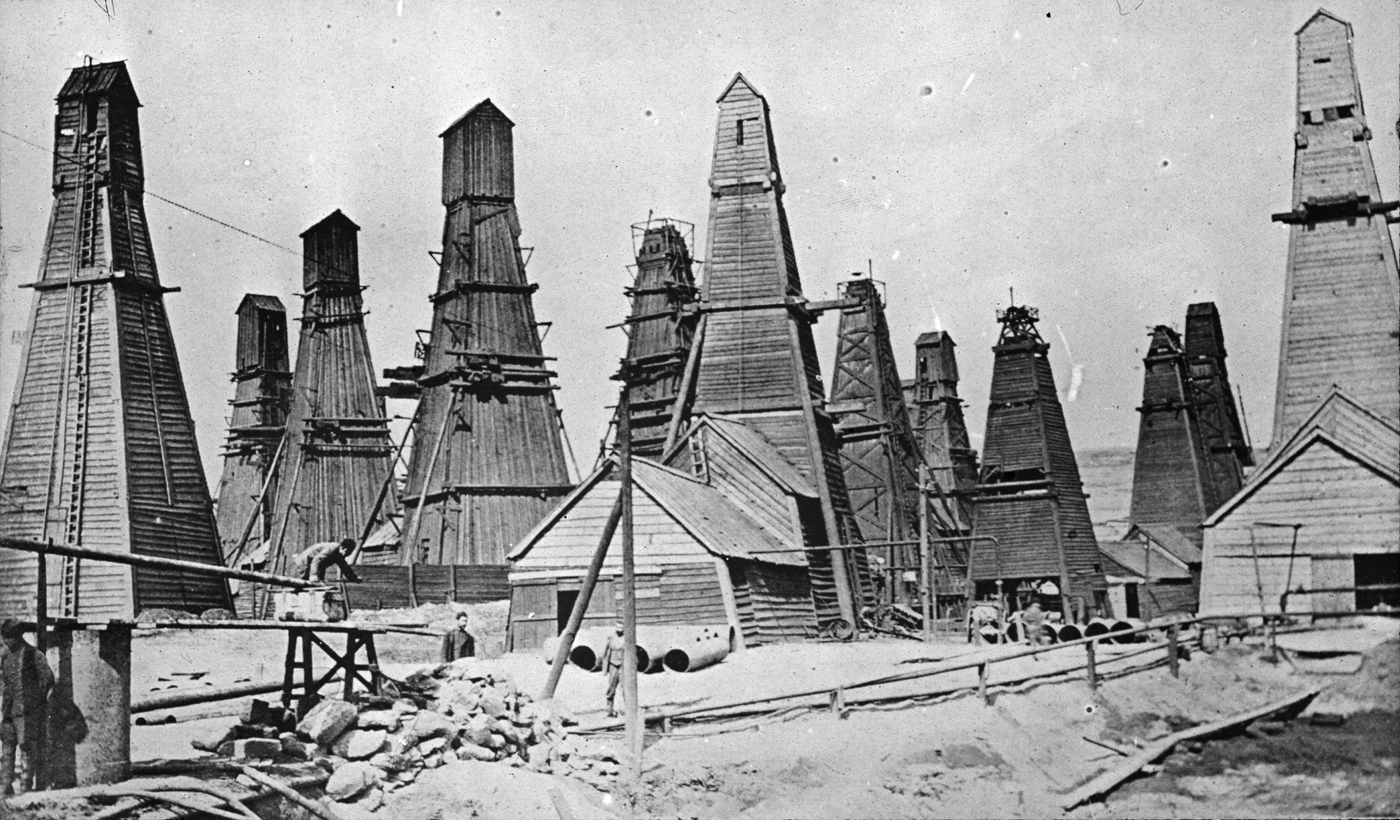
\includegraphics[width=0.33\textwidth]{balakhani_1904.png}
  \caption{Campos Balakhani (1904): infraestrutura de produção primitiva.}
  \label{fig:balakhani}
  \vspace{-0.5cm}
\end{wrapfigure}

Até o século XVIII, a exploração ocorria de forma rudimentar, sem conhecimento geológico ou métodos sistemáticos. A ausência de fundamentos científicos resultava em baixas taxas de recuperação e grande desperdício de recursos. Esta fase caracteriza-se por exploração artesanal, ausência de modelos físicos e produção baseada em tentativa e erro.

\section{Fundamentação Teórica (Séculos XIX e Início XX)}

A verdadeira revolução científica começou no século XIX com o surgimento da engenharia moderna. Em 1856, o engenheiro francês Henry Darcy formulou a lei que rege o escoamento de fluidos em meios porosos. A Lei de Darcy — expressa como $q = -k \frac{dP}{dx}$ — estabeleceu a base matemática da Engenharia de Reservatórios, permitindo quantificar a relação entre vazão, permeabilidade, viscosidade e gradiente de pressão.

\begin{wrapfigure}{l}{0.35\textwidth}
  \centering
  \vspace{-0.7cm}
  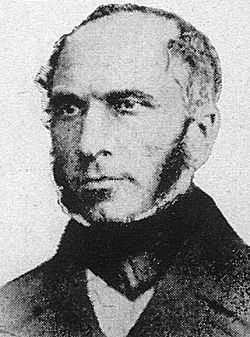
\includegraphics[width=0.33\textwidth]{Henry_Darcy.jpg}
  \caption{Henry Darcy (1803--1858): fundador da teoria do fluxo.}
  \label{fig:darcy}
  \vspace{-0.5cm}
\end{wrapfigure}

Em 1859, o poço Drake (Titusville, EUA) marcou o início da produção comercial de petróleo, impulsionando a exploração global. Essa combinação de fundamento teórico (Lei de Darcy) e viabilidade prática (Poço Drake) definiu o nascimento da Engenharia de Reservatórios como disciplina científica.

\section{Consolidação Científica (Século XX)}

O século XX marcou a transformação definitiva em disciplina estruturada. Pesquisadores como Muskat desenvolveram modelos matemáticos para fluxo multifásico. Os principais avanços incluem:

\textbf{Método do Balanço de Materiais:} permite estimar volume original de hidrocarbonetos e prever declínio de pressão durante produção.

\textbf{Análise de Pressão Transiente:} testes de pressão fornecem informações sobre permeabilidade, danos de formação e limites do reservatório.

\textbf{Simulação Numérica:} A introdução dos computadores representou ruptura paradigmática. Modelos tridimensionais integram dados geológicos, petrofísicos e operacionais, permitindo prever comportamento do campo antecipadamente.

\begin{figure}[H]
  \centering
  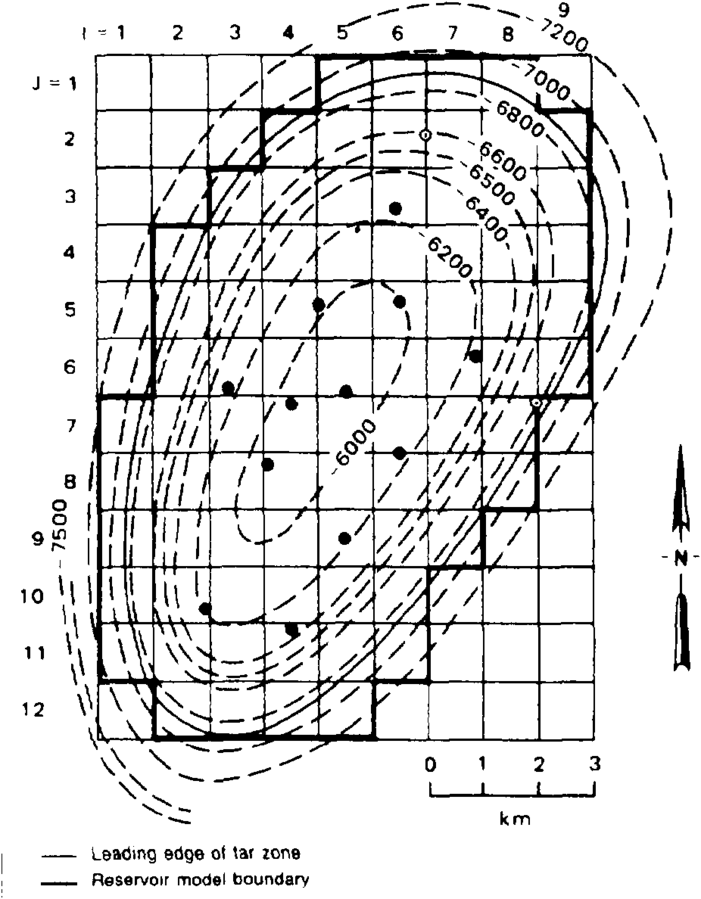
\includegraphics[width=0.50\textwidth]{701px-Conducting-a-reservoir-simulation-study-an-overview_fig3.png}
  \caption{Malha de simulação numérica: discretização para solver de equações multifásicas.}
  \label{fig:grid}
\end{figure}

\section{Era Digital (Século XXI)}

No século XXI, a Engenharia de Reservatórios entrou na era digital, caracterizada pela integração de tecnologias avançadas. Os principais desenvolvimentos incluem:

\textbf{Recuperação Avançada de Petróleo (EOR):} Métodos como injeção de gás, processos térmicos e métodos químicos aumentam fator de recuperação, tornando campos maduros economicamente viáveis novamente.

\textbf{Monitoramento em Tempo Real:} Sensores permanentes instalados em poços permitem coleta contínua de dados de pressão, temperatura e vazão, possibilitando otimização operacional imediata.

\textbf{Inteligência Artificial e Machine Learning:} Algoritmos modernos permitem prever curvas de declínio, otimizar produção automaticamente, identificar padrões em dados sísmicos e reduzir incertezas operacionais.

\begin{wrapfigure}{r}{0.35\textwidth}
  \centering
  \vspace{-0.7cm}
  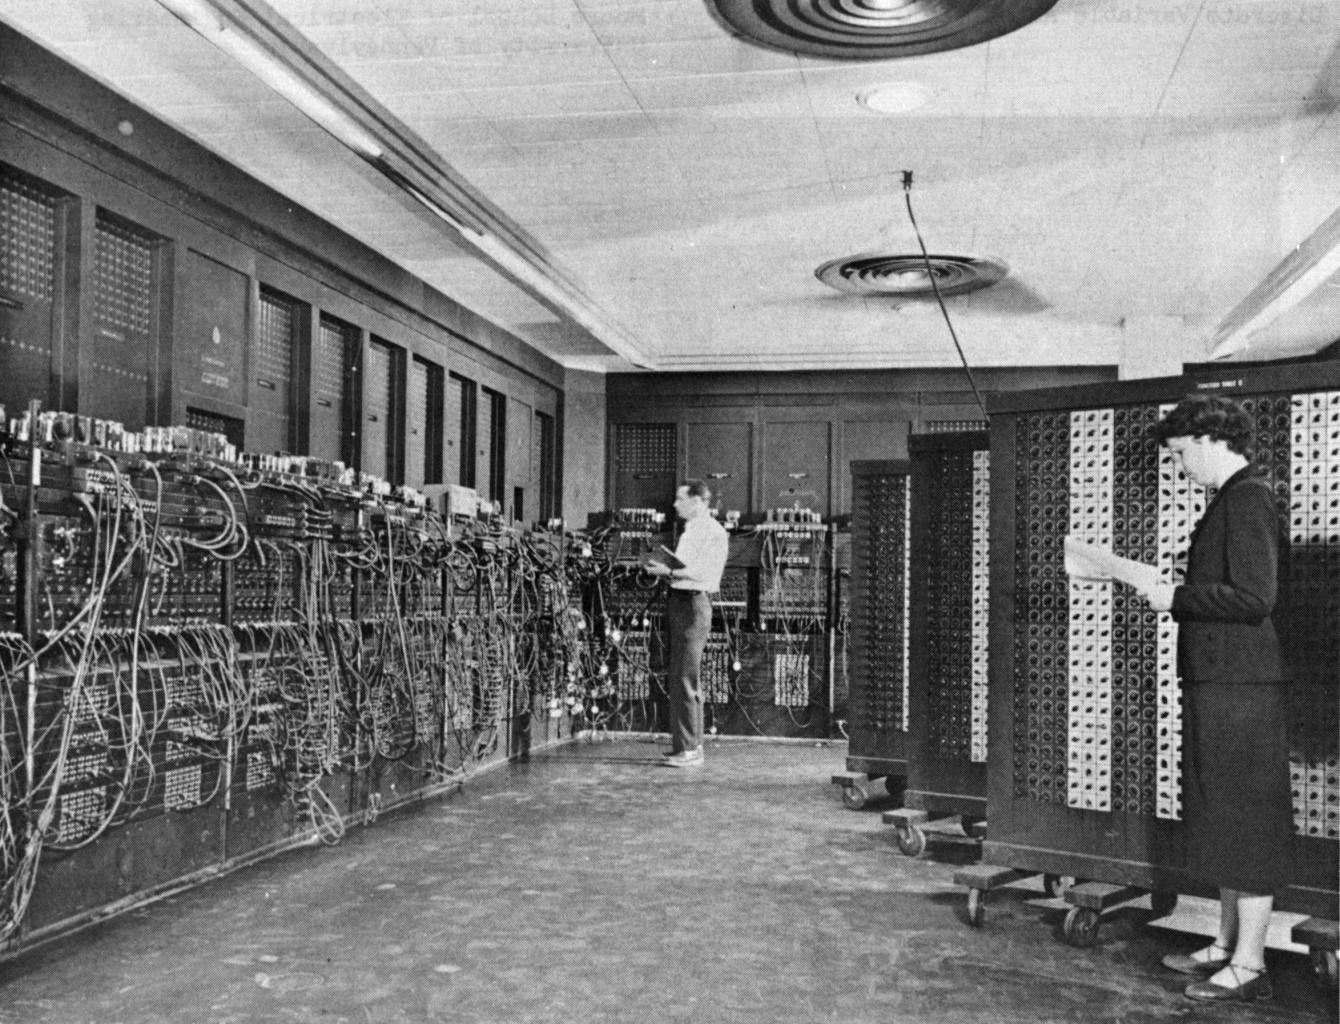
\includegraphics[width=0.33\textwidth]{eniac_1946.jpg}
  \caption{ENIAC (1946): primeira máquina de computação científica.}
  \label{fig:eniac}
  \vspace{-0.5cm}
\end{wrapfigure}

% ===========================
% CAPÍTULO 3: PROPRIEDADES FUNDAMENTAIS
% ===========================
\chapter{Propriedades Fundamentais de Rocha e Fluido}

O desempenho produtivo de um reservatório depende diretamente de suas propriedades petrofísicas.

\section{Porosidade e Permeabilidade}

\textbf{Porosidade} ($\phi$) mede o volume disponível para armazenamento de fluidos: $\phi = V_p / V_t$. A distinção entre porosidade total e efetiva (espaço poral interconectado) foi fundamental para compreensão de reservatórios.

\textbf{Permeabilidade} (k) indica a capacidade da rocha de permitir fluxo, expressa em Darcy ou milidarcies. A estrutura microscópica dos poros controla diretamente a produtividade do reservatório. A \textbf{permeabilidade relativa} descreve o comportamento de cada fase fluida quando múltiplas fases coexistem.

\section{Análise PVT e Classificação de Fluidos}

A análise Pressão-Volume-Temperatura (PVT) permite caracterizar comportamento termodinâmico dos fluidos, definindo estratégias de produção conforme o tipo: óleo negro, óleo volátil, gás condensado e gás seco. Os fluidos de reservatório são classificados em categorias dependendo de sua posição no diagrama PVT.

\textbf{Óleo Negro:} a maioria dos reservatórios; óleo escuro com gás dissolvido moderado.

\textbf{Óleo Volátil:} óleo mais leve; gás dissolvido significativo; queda maior de densidade com produção.

\textbf{Gás Condensado Retrógrado:} sistema gás dominante; líquido retrogradamente condensado durante produção.

% ===========================
% CAPÍTULO 4: APLICAÇÕES CONTEMPORÂNEAS
% ===========================
\chapter{Aplicações Contemporâneas e Perspectivas}

\section{Reservatórios Não Convencionais}

O avanço tecnológico possibilitou a produção em formações de baixa permeabilidade, como shale gas e tight oil, utilizando poços horizontais e fraturamento hidráulico. Esses recursos redefiniram o cenário energético global, aumentando reservas exploráveis.

\section{Engenharia de Reservatórios de Gás}

Reservatórios de gás apresentam comportamento distinto dos reservatórios de óleo devido à elevada compressibilidade do fluido, exigindo modelos específicos para previsão de produção e gerenciamento de pressão. A ausência de pressão diferencial significativa torna necessário desenvolvimento de técnicas diferenciadas.

\section{Captura e Armazenamento de CO\textsubscript{2} (CCS)}

A transição energética trouxe novos desafios ambientais. A tecnologia CCS consiste na injeção de dióxido de carbono em formações geológicas profundas, reduzindo emissões atmosféricas e utilizando conhecimentos típicos da Engenharia de Reservatórios. Esta aplicação representa uma ponte entre segurança energética e sustentabilidade ambiental.

% ===========================
% CAPÍTULO 5: SÍNTESE E CONCLUSÃO
% ===========================
\chapter{Síntese e Perspectivas Futuras}

A evolução da Engenharia de Reservatórios pode ser sintetizada em quatro eras principais:

\begin{enumerate}
  \item \textbf{Era Empírica} — exploração baseada exclusivamente na experiência prática;
  \item \textbf{Era Teórica} — surgimento da Lei de Darcy e fundamentos científicos;
  \item \textbf{Era de Consolidação Científica} — desenvolvimento de métodos analíticos e computacionais;
  \item \textbf{Era Digital} — integração de IA, IoT e simulação avançada.
\end{enumerate}

Essa trajetória demonstra a transformação da engenharia em ciência quantitativa altamente interdisciplinar. Para países produtores como Angola, dominar a Engenharia de Reservatórios significa maximizar recuperação de recursos, reduzir dependência tecnológica externa, aumentar eficiência econômica e garantir segurança energética.

A história da Engenharia de Reservatórios reflete a própria evolução da ciência aplicada. O campo evoluiu de práticas intuitivas para uma disciplina altamente tecnológica baseada em modelagem matemática, computação avançada e inteligência artificial.

Hoje, o engenheiro de reservatórios atua como gestor de sistemas físicos complexos, integrando geologia, física, matemática e ciência de dados para otimizar a produção de energia de forma eficiente e responsável. O futuro da área será marcado pela digitalização crescente, pela integração com tecnologias de baixo carbono e pela necessidade de equilibrar segurança energética e sustentabilidade ambiental. Nesse contexto, o domínio dessa disciplina torna-se fundamental para o desenvolvimento técnico e econômico de nações produtoras de petróleo.

\cleardoublepage
\printbibliography[title={Referências}]

\end{document}
